%TCIDATA{Version=5.50.0.2960}
%TCIDATA{LaTeXparent=0,0,abowd-schmutte-privacy-seminar.tex}

%TCIDATA{CSTFile=beamer.cst}

\section[Introduction]{Introduction}


%%%%%%%%%%%%%%%%%%%%%%%%%%%%%%%%%%%%%%%%%%%%%%%%%%%%%%%%%%%%%%%%%
%%%%%%%%%%%%%%%%%%%%%%%%%%%%%%%%%%%%%%%%%%%%%%%%%%%%%%%%%%%%%%%%%
%TCIMACRO{\TeXButton{BeginFrame}{\begin{frame}[allowframebreaks]}}%
%BeginExpansion
\begin{frame}[t]%
%EndExpansion
\frametitle{Production Possibilities}

\begin{onlyenv}<1-3>
	\begin{center}
		\includegraphics<1>[scale=.5]{blank}
		\includegraphics<2>[scale=.5]{MRT_1}
		\includegraphics<3>[scale=.5]{MRT_2}
	\end{center}
\end{onlyenv}


%TCIMACRO{\TeXButton{EndFrame}{\end{frame}}}%
%BeginExpansion
\end{frame}%
%EndExpansion
%
%%%%%%%%%%%%%%%%%%%%%%%%%%%%%%%%%%%%%%%%%%%%%%%%%%%%%%%%%%%%%%%%%
%%%%%%%%%%%%%%%%%%%%%%%%%%%%%%%%%%%%%%%%%%%%%%%%%%%%%%%%%%%%%%%%%








%%%%%%%%%%%%%%%%%%%%%%%%%%%%%%%%%%%%%%%%%%%%%%%%%%%%%%%%%%%%%%%%%
%%%%%%%%%%%%%%%%%%%%%%%%%%%%%%%%%%%%%%%%%%%%%%%%%%%%%%%%%%%%%%%%%
%TCIMACRO{\TeXButton{BeginFrame}{\begin{frame}[allowframebreaks]}}%
%BeginExpansion
\begin{frame}[allowframebreaks]%
%EndExpansion
\frametitle{Motivation}

\begin{itemize}
	\item Traditional Statistical Disclosure Limitation (SDL) methods affect all public-use data. \\(Abowd and Schmutte 2015; Alexander et al. 2010) \vspace{.25in}
	\item Privacy risk = residual disclosure (Fellegi 1972)
    \item Now called complementary disclosure or subtraction attack \vspace{.25in}
	\item SDL Methods:
	\begin{itemize}
		\item Coarsening
		\item Top-coding
		\item Item suppression (in cells, based on cell properties)
	\end{itemize}

\end{itemize}



%TCIMACRO{\TeXButton{EndFrame}{\end{frame}}}%
%BeginExpansion
\end{frame}%
%EndExpansion
%
%%%%%%%%%%%%%%%%%%%%%%%%%%%%%%%%%%%%%%%%%%%%%%%%%%%%%%%%%%%%%%%%%
%%%%%%%%%%%%%%%%%%%%%%%%%%%%%%%%%%%%%%%%%%%%%%%%%%%%%%%%%%%%%%%%%

%%%%%%%%%%%%%%%%%%%%%%%%%%%%%%%%%%%%%%%%%%%%%%%%%%%%%%%%%%%%%%%%%
%%%%%%%%%%%%%%%%%%%%%%%%%%%%%%%%%%%%%%%%%%%%%%%%%%%%%%%%%%%%%%%%%
%TCIMACRO{\TeXButton{BeginFrame}{\begin{frame}[allowframebreaks]}}%
%BeginExpansion
\begin{frame}[allowframebreaks]%
%EndExpansion
\frametitle{Motivation}

\begin{itemize}
	\item Modern SDL methods. \vspace{.25in}
	\item Privacy risk = inferential disclosure (Dalenius 1977, Duncan and Lambert 1986) \vspace{.25in}
	\item SDL methods and concepts
	\begin{itemize}
		\item Input/output noise infusion
		\item Synthetic data
		\item Differential privacy (form of output noise infusion) (Dwork 2006)
	\end{itemize}

	% \item Administrative and transaction databases proliferate providing both
	% \begin{itemize}
	% 	\item more, cheaper options for producing statistics;
	% 	\item greater risk of privacy loss.
	% \end{itemize}
\end{itemize}



%TCIMACRO{\TeXButton{EndFrame}{\end{frame}}}%
%BeginExpansion
\end{frame}%
%EndExpansion
%
%%%%%%%%%%%%%%%%%%%%%%%%%%%%%%%%%%%%%%%%%%%%%%%%%%%%%%%%%%%%%%%%%
%%%%%%%%%%%%%%%%%%%%%%%%%%%%%%%%%%%%%%%%%%%%%%%%%%%%%%%%%%%%%%%%%





%%%%%%%%%%%%%%%%%%%%%%%%%%%%%%%%%%%%%%%%%%%%%%%%%%%%%%%%%%%%%%%%%
%%%%%%%%%%%%%%%%%%%%%%%%%%%%%%%%%%%%%%%%%%%%%%%%%%%%%%%%%%%%%%%%%
%TCIMACRO{\TeXButton{BeginFrame}{\begin{frame}[allowframebreaks]}}%
%BeginExpansion
\begin{frame}[allowframebreaks]%
%EndExpansion
\frametitle{An Illustrative Solution to the Social Planner's Problem}

\begin{center}
	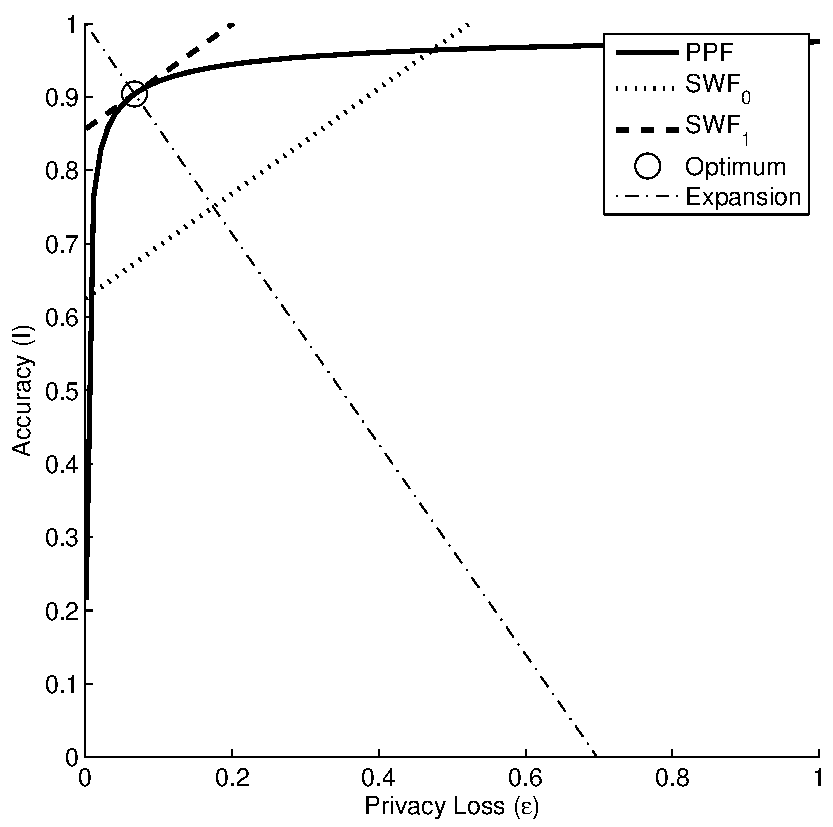
\includegraphics[scale=.5]{plannersprob_income}
\end{center}


%TCIMACRO{\TeXButton{EndFrame}{\end{frame}}}%
%BeginExpansion
\end{frame}%
%EndExpansion
%
%%%%%%%%%%%%%%%%%%%%%%%%%%%%%%%%%%%%%%%%%%%%%%%%%%%%%%%%%%%%%%%%%
%%%%%%%%%%%%%%%%%%%%%%%%%%%%%%%%%%%%%%%%%%%%%%%%%%%%%%%%%%%%%%%%%

%%%%%%%%%%%%%%%%%%%%%%%%%%%%%%%%%%%%%%%%%%%%%%%%%%%%%%%%%%%%%%%%%
%%%%%%%%%%%%%%%%%%%%%%%%%%%%%%%%%%%%%%%%%%%%%%%%%%%%%%%%%%%%%%%%%
%TCIMACRO{\TeXButton{BeginFrame}{\begin{frame}[allowframebreaks]}}%
%BeginExpansion
\begin{frame}[allowframebreaks]%
%EndExpansion
\frametitle{Antecedents}
\begin{itemize}
	\item Risk-Utility confidentiality maps (Duncan and Fienberg 1999; Duncan et al. 2011) \vspace*{.25in}
	\item Differential privacy in electronic commerce (McSherry and Talwar 2007; Ghosh and Roth 2011) \vspace*{.25in}
	\item Economics of privacy
	\begin{itemize}
		\item Stigler (1980); Posner (1981)
		\item Price discrimination (Acquisti and Varian 2005; Acquisti et al. 2013)
	\end{itemize}
\end{itemize}

%TCIMACRO{\TeXButton{EndFrame}{\end{frame}}}%
%BeginExpansion
\end{frame}%
%EndExpansion
%
%%%%%%%%%%%%%%%%%%%%%%%%%%%%%%%%%%%%%%%%%%%%%%%%%%%%%%%%%%%%%%%%%
%%%%%%%%%%%%%%%%%%%%%%%%%%%%%%%%%%%%%%%%%%%%%%%%%%%%%%%%%%%%%%%%%

%%%%%%%%%%%%%%%%%%%%%%%%%%%%%%%%%%%%%%%%%%%%%%%%%%%%%%%%%%%%%%%%%
%%%%%%%%%%%%%%%%%%%%%%%%%%%%%%%%%%%%%%%%%%%%%%%%%%%%%%%%%%%%%%%%%
%TCIMACRO{\TeXButton{BeginFrame}{\begin{frame}[allowframebreaks]}}%
%BeginExpansion
\begin{frame}[allowframebreaks]%
%EndExpansion
\frametitle{Contributions}
\begin{itemize}
    \item Formalization of algorithmic efficiency and the transformation set \vspace*{0.25in}
	\item Complete formalization of the idea behind R-U confidentiality map \vspace*{0.25in}
	\item Importance of public good nature of accuracy and privacy in existing EC models \vspace*{0.25in}
	\item Framework for optimal public decision-making in a world with massive databases
	
\end{itemize}


%TCIMACRO{\eXButton{EndFrame}{\end{frame}}}%
%BeginExpansion
\end{frame}%
%EndExpansionT




\section[Preliminaries]{Preliminaries}

%%%%%%%%%%%%%%%%%%%%%%%%%%%%%%%%%%%%%%%%%%%%%%%%%%%%%%%%%%%%%%%%%
%%%%%%%%%%%%%%%%%%%%%%%%%%%%%%%%%%%%%%%%%%%%%%%%%%%%%%%%%%%%%%%%%
%TCIMACRO{\TeXButton{BeginFrame}{\begin{frame}[allowframebreaks]}}%
%BeginExpansion
\begin{frame}[allowframebreaks]%
%EndExpansion

\begin{center}
	{\Large Basic Model of Data Publication}
\end{center}



%TCIMACRO{\TeXButton{EndFrame}{\end{frame}}}%
%BeginExpansion
\end{frame}%
%EndExpansion
%
%%%%%%%%%%%%%%%%%%%%%%%%%%%%%%%%%%%%%%%%%%%%%%%%%%%%%%%%%%%%%%%%%
%%%%%%%%%%%%%%%%%%%%%%%%%%%%%%%%%%%%%%%%%%%%%%%%%%%%%%%%%%%%%%%%%

%%%%%%%%%%%%%%%%%%%%%%%%%%%%%%%%%%%%%%%%%%%%%%%%%%%%%%%%%%%%%%%%%
%%%%%%%%%%%%%%%%%%%%%%%%%%%%%%%%%%%%%%%%%%%%%%%%%%%%%%%%%%%%%%%%%
%TCIMACRO{\TeXButton{BeginFrame}{\begin{frame}[allowframebreaks]}}%
%BeginExpansion
\begin{frame}[allowframebreaks]%
%EndExpansion
\frametitle{Overview}
\begin{itemize}
	\item Database represented as a histogram [contingency table] \vspace*{0.25in}
	\item Curator publishes answers to queries [table margins] \vspace*{0.25in}
	\item Randomized mechanism [output noise infusion] \vspace*{0.25in}
	\item Formal definitions of
	\begin{itemize}
		\item Privacy loss
		\item Accuracy
	\end{itemize}
\end{itemize}


%TCIMACRO{\TeXButton{EndFrame}{\end{frame}}}%
%BeginExpansion
\end{frame}%
%EndExpansion
%
%%%%%%%%%%%%%%%%%%%%%%%%%%%%%%%%%%%%%%%%%%%%%%%%%%%%%%%%%%%%%%%%%
%%%%%%%%%%%%%%%%%%%%%%%%%%%%%%%%%%%%%%%%%%%%%%%%%%%%%%%%%%%%%%%%%

%%%%%%%%%%%%%%%%%%%%%%%%%%%%%%%%%%%%%%%%%%%%%%%%%%%%%%%%%%%%%%%%%
%%%%%%%%%%%%%%%%%%%%%%%%%%%%%%%%%%%%%%%%%%%%%%%%%%%%%%%%%%%%%%%%%
%TCIMACRO{\TeXButton{BeginFrame}{\begin{frame}[allowframebreaks]}}%
%BeginExpansion
\begin{frame}[allowframebreaks]%
%EndExpansion
\frametitle{Histograms}
\begin{itemize}
	\item Database: an unnormalized histogram $x\in \mathbb{Z}^{\ast |\chi |}$
	\item $x_{i}$, is the count of elements in the database $D$ of type $i\in \chi $
	\item $||x||_{1}=\sum_{i=1}^{|\chi |}\left\vert x_{i}\right\vert$ .
	\item $||{x}-{y}||_{1}$: number of records that differ between ${x}$ and ${y}$
	\item $x$ and $y$ are \textit{adjacent} if $||{x}-{y}||_{1}=1$ \vspace*{.25in}
\end{itemize}

\textbf{Intuition:}
\begin{itemize}
	\item The database is a contingency table
	\item $\chi$ are cross-classifications of attributes


\end{itemize}


%TCIMACRO{\TeXButton{EndFrame}{\end{frame}}}%
%BeginExpansion
\end{frame}%
%EndExpansion
%
%%%%%%%%%%%%%%%%%%%%%%%%%%%%%%%%%%%%%%%%%%%%%%%%%%%%%%%%%%%%%%%%%
%%%%%%%%%%%%%%%%%%%%%%%%%%%%%%%%%%%%%%%%%%%%%%%%%%%%%%%%%%%%%%%%%

%%%%%%%%%%%%%%%%%%%%%%%%%%%%%%%%%%%%%%%%%%%%%%%%%%%%%%%%%%%%%%%%%
%%%%%%%%%%%%%%%%%%%%%%%%%%%%%%%%%%%%%%%%%%%%%%%%%%%%%%%%%%%%%%%%%
%TCIMACRO{\TeXButton{BeginFrame}{\begin{frame}[allowframebreaks]}}%
%BeginExpansion
\begin{frame}[allowframebreaks]%
%EndExpansion
\frametitle{Queries}
\begin{definition}{Linear Query}
A \textit{linear query} is a mapping $f:[-1,1]^{|\chi |}\times \mathbb{Z}%
^{\ast |\chi |}\rightarrow \mathbb{Z}^{\ast }$ such that $f(m,x)=m^{T}x$
where $x\in \mathbb{Z}^{\ast |\chi |}$ and $m\in \lbrack -1,1]^{|\chi |}$.
\end{definition}

\textbf{Intuition:}
\begin{itemize}
	\item \textit{Counting query:} $m_{i}\in\{0,1\}$
	\item The number of observations that satisfy particular conditions
	\item Can be used to calculate all margins of the contingency table
	\item \textit{Normalized Counting Queries:} Normalize output by database size; (a.k.a.\ proportions, not frequencies)
\end{itemize}
% A
% \textit{counting query} is a special case in which  Counting queries return . They are the tool an
% analyst would use to calculate multidimensional margins for the contingency
% table representation of the database. A \textit{normalized linear query} is
% a mapping $f:[-1,1]^{|\chi |}\times \mathbb{Z}^{\ast |\chi |}\rightarrow
% \lbrack 0,1]$ such that if $\tilde{f}$ is a linear query then $f(m,x)=\tilde{%
% f}(m,x)/||x||_{1}$.

%TCIMACRO{\TeXButton{EndFrame}{\end{frame}}}%
%BeginExpansion
\end{frame}%
%EndExpansion
%
%%%%%%%%%%%%%%%%%%%%%%%%%%%%%%%%%%%%%%%%%%%%%%%%%%%%%%%%%%%%%%%%%
%%%%%%%%%%%%%%%%%%%%%%%%%%%%%%%%%%%%%%%%%%%%%%%%%%%%%%%%%%%%%%%%%

%%%%%%%%%%%%%%%%%%%%%%%%%%%%%%%%%%%%%%%%%%%%%%%%%%%%%%%%%%%%%%%%%
%%%%%%%%%%%%%%%%%%%%%%%%%%%%%%%%%%%%%%%%%%%%%%%%%%%%%%%%%%%%%%%%%
%TCIMACRO{\TeXButton{BeginFrame}{\begin{frame}[allowframebreaks]}}%
%BeginExpansion
\begin{frame}[allowframebreaks]%
%EndExpansion
\frametitle{Query Release Mechanism}
\begin{definition}[Query Release Mechanism]
\label{def:query_mechanism} Let $\mathcal{F}$ be a set of normalized linear
queries with domain $[-1,1]^{|\chi |}\times \mathbb{Z}^{\ast |\chi |}$ and
range $R\subseteq \left[ 0,1\right] $, and let $k$ be the number of queries
to be answered. A query release mechanism $M$ is a random function $M:%
\mathbb{Z}^{\ast |\chi |}\times \mathcal{F}^{k}\rightarrow R^{k}$ whose
inputs are a histogram $x\in \mathbb{Z}^{\ast |\chi |}$ and a set of $k$
normalized linear queries $f=(f_{1},\ldots ,f_{k})\in \mathcal{F}^{k}$. The
probability of observing $B\subseteq R^{k}$ is $\Pr \left[ M(x,(f_{1},\ldots
,f_{k})\in B|X=x,F=f\right] $, where $\Pr \left[ z\in B|X=x,F=f\right] $ is
the conditional probability given $X=x$ and $F=f$ that the query output is
in $B\in \mathcal{B}$, where $\mathcal{B}$ are the measurable subsets of $%
R^{k}$.
\end{definition}


%TCIMACRO{\TeXButton{EndFrame}{\end{frame}}}%
%BeginExpansion
\end{frame}%
%EndExpansion
%
%%%%%%%%%%%%%%%%%%%%%%%%%%%%%%%%%%%%%%%%%%%%%%%%%%%%%%%%%%%%%%%%%
%%%%%%%%%%%%%%%%%%%%%%%%%%%%%%%%%%%%%%%%%%%%%%%%%%%%%%%%%%%%%%%%%



%%%%%%%%%%%%%%%%%%%%%%%%%%%%%%%%%%%%%%%%%%%%%%%%%%%%%%%%%%%%%%%%%
%%%%%%%%%%%%%%%%%%%%%%%%%%%%%%%%%%%%%%%%%%%%%%%%%%%%%%%%%%%%%%%%%
%TCIMACRO{\TeXButton{BeginFrame}{\begin{frame}[allowframebreaks]}}%
%BeginExpansion
\begin{frame}[allowframebreaks]%
%EndExpansion
\frametitle{Differential Privacy}
\begin{definition}[$(\protect\varepsilon ,\protect\delta )$-differential
privacy]
\label{def:dif_priv} A query release mechanism $M$ satisfies $(\varepsilon
,\delta )$-differential privacy if
\begin{equation*}
\sup_{x,x^{\prime }\in N_{x}}\sup_{B\in \mathcal{B}}\left\{ \frac{\Pr \left[
M(x,(f_{1},\ldots ,f_{k}))\in B\right] }{\Pr \left[ M(x^{\prime
},(f_{1},\ldots ,f_{k}))\in B\right] +\delta }\right\} \leq e^{\varepsilon },
\end{equation*}%
where $N_{x}=\left\{ (x,x^{\prime })\ s.t.~x,x^{\prime }\in \mathbb{Z}^{\ast
|\chi |}~\text{and}~||x-x^{\prime }||_{1}=1\right\} $ and $\mathcal{B}$ are
the measurable subsets of the query output space, $R^{k}$. The set $N_{x}$
contains all the \textit{adjacent histograms} of $x$.
\end{definition}

%TCIMACRO{\TeXButton{EndFrame}{\end{frame}}}%
%BeginExpansion
\end{frame}%
%EndExpansion
%
%%%%%%%%%%%%%%%%%%%%%%%%%%%%%%%%%%%%%%%%%%%%%%%%%%%%%%%%%%%%%%%%%
%%%%%%%%%%%%%%%%%%%%%%%%%%%%%%%%%%%%%%%%%%%%%%%%%%%%%%%%%%%%%%%%%

%%%%%%%%%%%%%%%%%%%%%%%%%%%%%%%%%%%%%%%%%%%%%%%%%%%%%%%%%%%%%%%%%
%%%%%%%%%%%%%%%%%%%%%%%%%%%%%%%%%%%%%%%%%%%%%%%%%%%%%%%%%%%%%%%%%
%TCIMACRO{\TeXButton{BeginFrame}{\begin{frame}[allowframebreaks]}}%
%BeginExpansion
\begin{frame}[allowframebreaks]%
%EndExpansion
\frametitle{Differential Privacy and Inferential Disclosure}
\begin{itemize}

\item Let $x$ and $x^{\prime }$ differ in one entry.
\item WLOG, $x$ and $x^{\prime }$ are $N$ samples from Multinomial with prob.\ $\pi $
\item By Bayes Theorem:
% \item Inferential disclosure occurs if
% $$\Pr \left[ X=x\left\vert \pi, N, F=f\right. \right]$$ and
% $\Pr \left[ X=x^{\prime}\left\vert \pi, N, F=f\right. \right]$.

\begin{equation*}
\frac{\Pr \left[ M(x,(f_{1},\ldots ,f_{k})\in B|X=x,F=f\right] }{\Pr \left[
M(x^{\prime },(f_{1},\ldots ,f_{k})\in B|X=x^{\prime },F=f\right] }=\frac{%
\frac{\Pr \left[ X=x\left\vert B,\pi ,N,F=f\right. \right] }{\Pr \left[
X=x^{\prime }\left\vert B,\pi ,N,F=f\right. \right] }}{\frac{\Pr \left[
X=x\left\vert \pi ,N,F=f\right. \right] }{\Pr \left[ X=x^{\prime }\left\vert
\pi ,N,F=f\right. \right] }},  \label{eq:posterior_odds}
\end{equation*}%
\item LHS is $(\varepsilon,0)$-differential privacy
\item RHS is the posterior odds for the confidential data after v. before release.
\item Implications
\begin{enumerate}
	\item Differential privacy bounds ability to distinguish inputs based on output
	\item No information can be released without some privacy loss [impossibility of zero inferential disclosure]
\end{enumerate}
\end{itemize}
%TCIMACRO{\TeXButton{EndFrame}{\end{frame}}}%
%BeginExpansion
\end{frame}%
%EndExpansion
%
%%%%%%%%%%%%%%%%%%%%%%%%%%%%%%%%%%%%%%%%%%%%%%%%%%%%%%%%%%%%%%%%%
%%%%%%%%%%%%%%%%%%%%%%%%%%%%%%%%%%%%%%%%%%%%%%%%%%%%%%%%%%%%%%%%%



%%%%%%%%%%%%%%%%%%%%%%%%%%%%%%%%%%%%%%%%%%%%%%%%%%%%%%%%%%%%%%%%%
%%%%%%%%%%%%%%%%%%%%%%%%%%%%%%%%%%%%%%%%%%%%%%%%%%%%%%%%%%%%%%%%%
%TCIMACRO{\TeXButton{BeginFrame}{\begin{frame}[allowframebreaks]}}%
%BeginExpansion
\begin{frame}[allowframebreaks]%
%EndExpansion
\frametitle{Accuracy}
\begin{definition}[$(\protect\alpha ,\protect\beta )$-accuracy]
\label{def:acc} A query release mechanism $M$ satisfies $(\alpha ,\beta )$%
-accuracy for query sequence $\left\{ f_{1},f_{2},\ldots ,f_{k}\right\} \in
\mathcal{F}^{k}$, $0<\alpha \leq 1$, and $0<\beta \leq 1$, if
$$\min_{1\leq i\leq k}\left\{ \Pr \left[ |a_{i}-f_{i}(x)|\leq \alpha \right] \right\} \geq
1-\beta. $$%
\end{definition}

%TCIMACRO{\TeXButton{EndFrame}{\end{frame}}}%
%BeginExpansion
\end{frame}%
%EndExpansion
%
%%%%%%%%%%%%%%%%%%%%%%%%%%%%%%%%%%%%%%%%%%%%%%%%%%%%%%%%%%%%%%%%%
%%%%%%%%%%%%%%%%%%%%%%%%%%%%%%%%%%%%%%%%%%%%%%%%%%%%%%%%%%%%%%%%%

\section[Suboptimality]{Suboptimality}

%%%%%%%%%%%%%%%%%%%%%%%%%%%%%%%%%%%%%%%%%%%%%%%%%%%%%%%%%%%%%%%%%
%%%%%%%%%%%%%%%%%%%%%%%%%%%%%%%%%%%%%%%%%%%%%%%%%%%%%%%%%%%%%%%%%
%TCIMACRO{\TeXButton{BeginFrame}{\begin{frame}[allowframebreaks]}}%
%BeginExpansion
\begin{frame}[allowframebreaks]%
%EndExpansion

\begin{center}
	{\Large Model 1: Suboptimality of Private Provision}
\end{center}



%TCIMACRO{\TeXButton{EndFrame}{\end{frame}}}%
%BeginExpansion
\end{frame}%
%EndExpansion
%
%%%%%%%%%%%%%%%%%%%%%%%%%%%%%%%%%%%%%%%%%%%%%%%%%%%%%%%%%%%%%%%%%
%%%%%%%%%%%%%%%%%%%%%%%%%%%%%%%%%%%%%%%%%%%%%%%%%%%%%%%%%%%%%%%%%

%%%%%%%%%%%%%%%%%%%%%%%%%%%%%%%%%%%%%%%%%%%%%%%%%%%%%%%%%%%%%%%%%
%%%%%%%%%%%%%%%%%%%%%%%%%%%%%%%%%%%%%%%%%%%%%%%%%%%%%%%%%%%%%%%%%
%TCIMACRO{\TeXButton{BeginFrame}{\begin{frame}[allowframebreaks]}}%
%BeginExpansion
\begin{frame}[allowframebreaks]%
%EndExpansion
\frametitle{Simplified Definitions}
\begin{itemize}
	\item Data quality: $I=1-\alpha$, $0<I<1$ \vspace*{.25in}
	\item Privacy loss: $\varepsilon$, $0<\varepsilon<1$ \vspace*{.25in}
	\item Data quality, $I$, is a public good \vspace*{.25in}
	\item Privacy loss, $\varepsilon$, is a public bad \vspace*{.25in}
	\item The preferences of consumer $i$ are
		\begin{equation}
		v_{i}\left( y_{i},\varepsilon,I \right) =\ln y_{i}+p_{\varepsilon
		}\varepsilon -\gamma _{i}\varepsilon +\eta _{i}I-p_II_{i}  %\label{eqn:linear2}
		\end{equation}%
	\item Utility of privacy loss: $\left(p_{\varepsilon}-\gamma_{i}\right)\varepsilon$
	\item Utility of data quality: $\eta_{i}I-p_II_{i}$ \vspace*{.25in}
\end{itemize}


%TCIMACRO{\TeXButton{EndFrame}{\end{frame}}}%
%BeginExpansion
\end{frame}%
%EndExpansion
%
%%%%%%%%%%%%%%%%%%%%%%%%%%%%%%%%%%%%%%%%%%%%%%%%%%%%%%%%%%%%%%%%%
%%%%%%%%%%%%%%%%%%%%%%%%%%%%%%%%%%%%%%%%%%%%%%%%%%%%%%%%%%%%%%%%%

%%%%%%%%%%%%%%%%%%%%%%%%%%%%%%%%%%%%%%%%%%%%%%%%%%%%%%%%%%%%%%%%%
%%%%%%%%%%%%%%%%%%%%%%%%%%%%%%%%%%%%%%%%%%%%%%%%%%%%%%%%%%%%%%%%%
%TCIMACRO{\TeXButton{BeginFrame}{\begin{frame}[allowframebreaks]}}%
%BeginExpansion
\begin{frame}[allowframebreaks]%
%EndExpansion
\frametitle{Data Publication Problem}
\begin{itemize}
	\item Data custodian possesses a single bit, $b_{i}$, of information on $N$ individuals
	\item \textbf{Goal:} produce an $\left( \alpha,\beta \right) $-accurate estimate $\hat{s}$ of the population
statistic%
\begin{equation}
s=\frac{1}{N}\sum_{i=1}^{N}b_{i}  \label{eqn:s_def}
\end{equation}%
\item \textbf{Technology: } GR prove that
to produce $\hat{s}$ with $\left( \alpha ,1/3\right) $-accuracy requires $\varepsilon =\frac{1/2+\ln 3}{\alpha N}$ units of privacy loss from $H=N-\frac{\alpha N}{%
1/2+\ln 3}$ members of the database
\end{itemize}



%TCIMACRO{\TeXButton{EndFrame}{\end{frame}}}%
%BeginExpansion
\end{frame}%
%EndExpansion
%
%%%%%%%%%%%%%%%%%%%%%%%%%%%%%%%%%%%%%%%%%%%%%%%%%%%%%%%%%%%%%%%%%
%%%%%%%%%%%%%%%%%%%%%%%%%%%%%%%%%%%%%%%%%%%%%%%%%%%%%%%%%%%%%%%%%


\section[Suboptimality]{Suboptimality}

%%%%%%%%%%%%%%%%%%%%%%%%%%%%%%%%%%%%%%%%%%%%%%%%%%%%%%%%%%%%%%%%%
%%%%%%%%%%%%%%%%%%%%%%%%%%%%%%%%%%%%%%%%%%%%%%%%%%%%%%%%%%%%%%%%%
%TCIMACRO{\TeXButton{BeginFrame}{\begin{frame}[allowframebreaks]}}%
%BeginExpansion
\begin{frame}[allowframebreaks]%
%EndExpansion

\begin{center}
	{\Large Model 1: Suboptimality of Private Provision}
\end{center}



%TCIMACRO{\TeXButton{EndFrame}{\end{frame}}}%
%BeginExpansion
\end{frame}%
%EndExpansion
%
%%%%%%%%%%%%%%%%%%%%%%%%%%%%%%%%%%%%%%%%%%%%%%%%%%%%%%%%%%%%%%%%%
%%%%%%%%%%%%%%%%%%%%%%%%%%%%%%%%%%%%%%%%%%%%%%%%%%%%%%%%%%%%%%%%%

%%%%%%%%%%%%%%%%%%%%%%%%%%%%%%%%%%%%%%%%%%%%%%%%%%%%%%%%%%%%%%%%%
%%%%%%%%%%%%%%%%%%%%%%%%%%%%%%%%%%%%%%%%%%%%%%%%%%%%%%%%%%%%%%%%%
%TCIMACRO{\TeXButton{BeginFrame}{\begin{frame}[allowframebreaks]}}%
%BeginExpansion
\begin{frame}[allowframebreaks]%
%EndExpansion
\frametitle{A Model of Private Provision}
Based on Ghosh and Roth (2011)
\begin{enumerate}
	\item $\varepsilon$-DP can be priced through a procurement auction
	\item A VCG auction yields minimum-cost method for answering a query with
	\begin{itemize}
		\item $\left( \varepsilon ,0\right) $-differential privacy
		\item $\left(\alpha ,\beta \right) $-accuracy
	\end{itemize}
	\item \textbf{Minimum Cost Procurement:} Purchasing the data-use rights from the $H$ least
privacy-loving members of the population; \textit{i.e.}, those with the
smallest $\gamma _{i}$, is the minimum-cost, envy-free implementation
mechanism
\end{enumerate}


%TCIMACRO{\TeXButton{EndFrame}{\end{frame}}}%
%BeginExpansion
\end{frame}%
%EndExpansion
%
%%%%%%%%%%%%%%%%%%%%%%%%%%%%%%%%%%%%%%%%%%%%%%%%%%%%%%%%%%%%%%%%%
%%%%%%%%%%%%%%%%%%%%%%%%%%%%%%%%%%%%%%%%%%%%%%%%%%%%%%%%%%%%%%%%%

%%%%%%%%%%%%%%%%%%%%%%%%%%%%%%%%%%%%%%%%%%%%%%%%%%%%%%%%%%%%%%%%%
%%%%%%%%%%%%%%%%%%%%%%%%%%%%%%%%%%%%%%%%%%%%%%%%%%%%%%%%%%%%%%%%%
%TCIMACRO{\TeXButton{BeginFrame}{\begin{frame}[allowframebreaks]}}%
%BeginExpansion
\begin{frame}[allowframebreaks]%
%EndExpansion
\frametitle{Our Extension: The Demand for Statistical Accuracy}
\begin{itemize}
	\item Ghosh and Roth (2011) take the level of accuracy as exogenous.
	\item We model the supply decision of a private private profit-maximizing, price-taking, firm
	\item The firm sells $\hat{s}$ with data quality $I$ at price per unit of quality, $p$
	\item Profits:%
\begin{equation*}
P\left( I\right) =pI-C^{VCG}(I)
\end{equation*}%
where
\begin{equation}
C^{VCG}(I)=Q\left( \frac{H(I)}{N}\right) H(I)\varepsilon (I)
\label{eqn:c_def}
\end{equation}%
and
\begin{equation}
\varepsilon (I)=\frac{1/2+\ln 3}{(1-I)N}  \label{eqn:e_def}
\end{equation}

% \item First order condition:
% {\small
% \begin{equation*}
% p= Q\left( \frac{H(I)}{N}\right) H(I)\varepsilon ^{\prime }(I)+\left[ Q\left(
% \frac{H(I)}{N}\right) +Q^{\prime }\left( \frac{H(I)}{N}\right) \left( \frac{%
% H(I)}{N}\right) \right] H^{\prime }(I)\varepsilon (I)  \label{eq:p_private}
% \end{equation*}
% }

% ($Q$ is the quantile function with respect to the population distribution of privacy preferences, $F_{\gamma }$)
% \end{itemize}

%TCIMACRO{\TeXButton{EndFrame}{\end{frame}}}%
%BeginExpansion
\end{frame}%
%EndExpansion
%
%%%%%%%%%%%%%%%%%%%%%%%%%%%%%%%%%%%%%%%%%%%%%%%%%%%%%%%%%%%%%%%%%
%%%%%%%%%%%%%%%%%%%%%%%%%%%%%%%%%%%%%%%%%%%%%%%%%%%%%%%%%%%%%%%%%

%%%%%%%%%%%%%%%%%%%%%%%%%%%%%%%%%%%%%%%%%%%%%%%%%%%%%%%%%%%%%%%%%
%%%%%%%%%%%%%%%%%%%%%%%%%%%%%%%%%%%%%%%%%%%%%%%%%%%%%%%%%%%%%%%%%
%TCIMACRO{\TeXButton{BeginFrame}{\begin{frame}[allowframebreaks]}}%
%BeginExpansion
\begin{frame}[allowframebreaks]%
%EndExpansion
\frametitle{Suboptimality of Private Provision}
\begin{theorem}
\label{theorem:suboptimality}$%
I^{VCG}\leq I^{L}\leq I^{0}$, where $I^{0}$ is the Pareto optimal level of $%
I $ , $I^{L}$
is the privately-provided level when using the Lindahl mechanism to procure
data-use rights and $I^{VCG}$ is the privately-provided level when using the
VCG\ procurement mechanism

\end{theorem}


%TCIMACRO{\TeXButton{EndFrame}{\end{frame}}}%
%BeginExpansion
\end{frame}%
%EndExpansion
%
%%%%%%%%%%%%%%%%%%%%%%%%%%%%%%%%%%%%%%%%%%%%%%%%%%%%%%%%%%%%%%%%%
%%%%%%%%%%%%%%%%%%%%%%%%%%%%%%%%%%%%%%%%%%%%%%%%%%%%%%%%%%%%%%%%%



%%%%%%%%%%%%%%%%%%%%%%%%%%%%%%%%%%%%%%%%%%%%%%%%%%%%%%%%%%%%%%%%%
%%%%%%%%%%%%%%%%%%%%%%%%%%%%%%%%%%%%%%%%%%%%%%%%%%%%%%%%%%%%%%%%%
%TCIMACRO{\TeXButton{BeginFrame}{\begin{frame}[allowframebreaks]}}%
%BeginExpansion
\begin{frame}[allowframebreaks]%
%EndExpansion
\frametitle{Suboptimality of Private Provision}
The Pareto optimal consumption of data quality, $I^{0},$ solves
\begin{equation}
\sum_{i=1}^{N}\eta _{i}=\frac{dC^{VCG}\left( I^{0}\right) }{dI}
\label{eqn:pareto_optimality}
\end{equation}%

%TCIMACRO{\TeXButton{EndFrame}{\end{frame}}}%
%BeginExpansion
\end{frame}%
%EndExpansion
%
%%%%%%%%%%%%%%%%%%%%%%%%%%%%%%%%%%%%%%%%%%%%%%%%%%%%%%%%%%%%%%%%%
%%%%%%%%%%%%%%%%%%%%%%%%%%%%%%%%%%%%%%%%%%%%%%%%%%%%%%%%%%%%%%%%%



%%%%%%%%%%%%%%%%%%%%%%%%%%%%%%%%%%%%%%%%%%%%%%%%%%%%%%%%%%%%%%%%%
%%%%%%%%%%%%%%%%%%%%%%%%%%%%%%%%%%%%%%%%%%%%%%%%%%%%%%%%%%%%%%%%%
%TCIMACRO{\TeXButton{BeginFrame}{\begin{frame}[allowframebreaks]}}%
%BeginExpansion
\begin{frame}[allowframebreaks]%
%EndExpansion
\frametitle{Our Extension: The Demand for Statistical Accuracy III}
\begin{itemize}
	
	\item At market price $p_I$, consumer $i$'s incremental accuracy, $I_{i}$ is the extra accuracy that she would pay for
    \item It is given by solving%
\begin{equation}
\max_{I_{i}\geq 0}\eta _{i}\left( I_{-i}+I_{i}\right) -p_II_{i}
%\label{eqn:umax}
\end{equation}%
    \item $I_{-i}$ is the amount $i$ gets when paying 0
    \item Classic free-rider game
	\item The equilibrium price and data quality will satisfy%
\begin{equation*}
p_I=\bar{\eta}=\frac{dC^{VCG}\left( I^{VCG}\right) }{dI}
\end{equation*}%
where $\bar{\eta}$ is the population maximum taste for accuracy
\end{itemize}



%TCIMACRO{\TeXButton{EndFrame}{\end{frame}}}%
%BeginExpansion
\end{frame}%
%EndExpansion
%
%%%%%%%%%%%%%%%%%%%%%%%%%%%%%%%%%%%%%%%%%%%%%%%%%%%%%%%%%%%%%%%%%
%%%%%%%%%%%%%%%%%%%%%%%%%%%%%%%%%%%%%%%%%%%%%%%%%%%%%%%%%%%%%%%%%



%%%%%%%%%%%%%%%%%%%%%%%%%%%%%%%%%%%%%%%%%%%%%%%%%%%%%%%%%%%%%%%%%
%%%%%%%%%%%%%%%%%%%%%%%%%%%%%%%%%%%%%%%%%%%%%%%%%%%%%%%%%%%%%%%%%
%TCIMACRO{\TeXButton{BeginFrame}{\begin{frame}[allowframebreaks]}}%
%BeginExpansion
\begin{frame}[allowframebreaks]%
%EndExpansion
\frametitle{Simplified PMW}
\begin{itemize}
	\item Answer first query using true data, adding noise ($a_t$)
	\item Answer first query using synthetic database ($\tilde{a}_t$)
	\item If $\tilde{a}_t$ is accurate enough, release
	\item Otherwise, release $a_t$ and update the synthetic database
	\item Iterate until query budget is exhausted
\end{itemize}

%TCIMACRO{\TeXButton{EndFrame}{\end{frame}}}%
%BeginExpansion
\end{frame}%
%EndExpansion
%
%%%%%%%%%%%%%%%%%%%%%%%%%%%%%%%%%%%%%%%%%%%%%%%%%%%%%%%%%%%%%%%%%
%%%%%%%%%%%%%%%%%%%%%%%%%%%%%%%%%%%%%%%%%%%%%%%%%%%%%%%%%%%%%%%%%

%%%%%%%%%%%%%%%%%%%%%%%%%%%%%%%%%%%%%%%%%%%%%%%%%%%%%%%%%%%%%%%%%
%%%%%%%%%%%%%%%%%%%%%%%%%%%%%%%%%%%%%%%%%%%%%%%%%%%%%%%%%%%%%%%%%
%TCIMACRO{\TeXButton{BeginFrame}{\begin{frame}[allowframebreaks]}}%
%BeginExpansion
\begin{frame}[allowframebreaks]%
%EndExpansion
\frametitle{Algorithmic Model of the Transformation Set}

\begin{theorem}
\label{thm:ppf} Let $D$ be a confidential database with rows from the set $\chi $ and histogram $x$ from population size $%
\left\Vert x\right\Vert _{1}=N$. The set of allowable normalized
linear queries is $\mathcal{Q\subseteq F}$.
Given parameters $\varepsilon >0$, $0<\delta <1$ and $0<\beta <1$, there
exist mechanisms $M(x)$ including the PMW mechanism that can
interactively answer sequences of queries $f_{t}\in \mathcal{Q}$ for $%
t=1,\ldots ,|\mathcal{Q}|$ such that:

\begin{enumerate}
\item Privacy: $M(x)$ satisfies $(\varepsilon ,\delta )$-differential
privacy;

\item Accuracy: $M(x)$ satisfies $(\alpha ,\beta )$-accuracy, with
\begin{equation}
\alpha =\frac{K(\delta ,\beta ,|\chi |,|\mathcal{Q}|,N)}{\varepsilon ^{b}},b \leq \frac{1}{2}
%\label{eqn:alpha_PMW}
\end{equation}%
% Furthermore, $K$ is decreasing in $N$, $\delta $,
% and $\beta $, and increasing in $|\chi |$ and $|\mathcal{Q}|$.
\end{enumerate}
\end{theorem}

%TCIMACRO{\TeXButton{EndFrame}{\end{frame}}}%
%BeginExpansion
\end{frame}%
%EndExpansion
%
%%%%%%%%%%%%%%%%%%%%%%%%%%%%%%%%%%%%%%%%%%%%%%%%%%%%%%%%%%%%%%%%%
%%%%%%%%%%%%%%%%%%%%%%%%%%%%%%%%%%%%%%%%%%%%%%%%%%%%%%%%%%%%%%%%%


%%%%%%%%%%%%%%%%%%%%%%%%%%%%%%%%%%%%%%%%%%%%%%%%%%%%%%%%%%%%%%%%%
%%%%%%%%%%%%%%%%%%%%%%%%%%%%%%%%%%%%%%%%%%%%%%%%%%%%%%%%%%%%%%%%%
%TCIMACRO{\TeXButton{BeginFrame}{\begin{frame}[allowframebreaks]}}%
%BeginExpansion
\begin{frame}[allowframebreaks]%
%EndExpansion
\frametitle{Production Possibilities Frontier}
% The production possibilities frontier (PPF) relating information quality $%
% I=(1-\alpha )$ and differential privacy loss $\varepsilon $ is defined by a
% transformation function%
% \begin{equation}
% G\left( \varepsilon ,I\right) \equiv I-\left[ 1-\frac{K(\delta ,\beta ,|\chi
% |,|\mathcal{Q}|,N)}{\varepsilon ^{b}}\right]
% \label{eqn:transformation_function}
% \end{equation}%
% % where Theorem \ref{thm:ppf} gives the functional form.
% All feasible pairs $%
% \left( \varepsilon ,I\right) $ are contained in the transformation set
% \begin{equation}
% Y=\left\{ \left( \varepsilon ,I\right) \left\vert \varepsilon >0,0<I<1\text{
% s.t. }G(\varepsilon ,I)\leq 0\right. \right\} .
% \label{eqn:transformation_set}
% \end{equation}%
The PPF is
\begin{equation}
PPF\left( \varepsilon ,I\right) =\left\{ \left( \varepsilon ,I\right)
\left\vert \varepsilon >0,0<I<1\text{ s.t. }G(\varepsilon ,I)=0\right. \right\}
\end{equation}%

\begin{equation}
I\left( \varepsilon ;\delta ,\beta ,|\chi |,|\mathcal{Q}|,N\right) =\left[ 1-%
\frac{K(\delta ,\beta ,|\chi |,|\mathcal{Q}|,N)}{\varepsilon ^{b}}\right]
%\label{eqn:difpriv}
\end{equation}%

%TCIMACRO{\TeXButton{EndFrame}{\end{frame}}}%
%BeginExpansion
\end{frame}%
%EndExpansion
%
%%%%%%%%%%%%%%%%%%%%%%%%%%%%%%%%%%%%%%%%%%%%%%%%%%%%%%%%%%%%%%%%%
%%%%%%%%%%%%%%%%%%%%%%%%%%%%%%%%%%%%%%%%%%%%%%%%%%%%%%%%%%%%%%%%%

%%%%%%%%%%%%%%%%%%%%%%%%%%%%%%%%%%%%%%%%%%%%%%%%%%%%%%%%%%%%%%%%%
%%%%%%%%%%%%%%%%%%%%%%%%%%%%%%%%%%%%%%%%%%%%%%%%%%%%%%%%%%%%%%%%%
%TCIMACRO{\TeXButton{BeginFrame}{\begin{frame}[allowframebreaks]}}%
%BeginExpansion
\begin{frame}[allowframebreaks]%
%EndExpansion
\frametitle{Marginal Rate of Transformation}
\begin{equation}
MRT\left( \varepsilon ,I\right) \equiv \frac{dI}{d\varepsilon } = -\frac{\partial G/\partial \varepsilon
}{\partial G/\partial I}=\frac{bK(\delta ,\beta ,|\chi |,|\mathcal{Q}|,N)}{%
\varepsilon ^{b+1}}%\label{eqn:MRT}
\end{equation}

%TCIMACRO{\TeXButton{EndFrame}{\end{frame}}}%
%BeginExpansion
\end{frame}%
%EndExpansion
%
%%%%%%%%%%%%%%%%%%%%%%%%%%%%%%%%%%%%%%%%%%%%%%%%%%%%%%%%%%%%%%%%%
%%%%%%%%%%%%%%%%%%%%%%%%%%%%%%%%%%%%%%%%%%%%%%%%%%%%%%%%%%%%%%%%%

% %%%%%%%%%%%%%%%%%%%%%%%%%%%%%%%%%%%%%%%%%%%%%%%%%%%%%%%%%%%%%%%%%
% %%%%%%%%%%%%%%%%%%%%%%%%%%%%%%%%%%%%%%%%%%%%%%%%%%%%%%%%%%%%%%%%%
% %TCIMACRO{\TeXButton{BeginFrame}{\begin{frame}[allowframebreaks]}}%
% %BeginExpansion
% \begin{frame}[allowframebreaks]%
% %EndExpansion
% \frametitle{}

% %TCIMACRO{\TeXButton{EndFrame}{\end{frame}}}%
% %BeginExpansion
% \end{frame}%
% %EndExpansion
% %
% %%%%%%%%%%%%%%%%%%%%%%%%%%%%%%%%%%%%%%%%%%%%%%%%%%%%%%%%%%%%%%%%%
% %%%%%%%%%%%%%%%%%%%%%%%%%%%%%%%%%%%%%%%%%%%%%%%%%%%%%%%%%%%%%%%%%

% %%%%%%%%%%%%%%%%%%%%%%%%%%%%%%%%%%%%%%%%%%%%%%%%%%%%%%%%%%%%%%%%%
% %%%%%%%%%%%%%%%%%%%%%%%%%%%%%%%%%%%%%%%%%%%%%%%%%%%%%%%%%%%%%%%%%
% %TCIMACRO{\TeXButton{BeginFrame}{\begin{frame}[allowframebreaks]}}%
% %BeginExpansion
% \begin{frame}[allowframebreaks]%
% %EndExpansion
% \frametitle{}

% %TCIMACRO{\TeXButton{EndFrame}{\end{frame}}}%
% %BeginExpansion
% \end{frame}%
% %EndExpansion
% %
% %%%%%%%%%%%%%%%%%%%%%%%%%%%%%%%%%%%%%%%%%%%%%%%%%%%%%%%%%%%%%%%%%
% %%%%%%%%%%%%%%%%%%%%%%%%%%%%%%%%%%%%%%%%%%%%%%%%%%%%%%%%%%%%%%%%%





%%%%%%%%%%%%%%%%%%%%%%%%%%%%%%%%%%%%%%%%%%%%%%%%%%%%%%%%%%%%%%%%%
%%%%%%%%%%%%%%%%%%%%%%%%%%%%%%%%%%%%%%%%%%%%%%%%%%%%%%%%%%%%%%%%%
%TCIMACRO{\TeXButton{BeginFrame}{\begin{frame}[allowframebreaks]}}%
%BeginExpansion
\begin{frame}[allowframebreaks]%
%EndExpansion
\frametitle{Solution to the Social Planner's Problem}

\begin{center}
	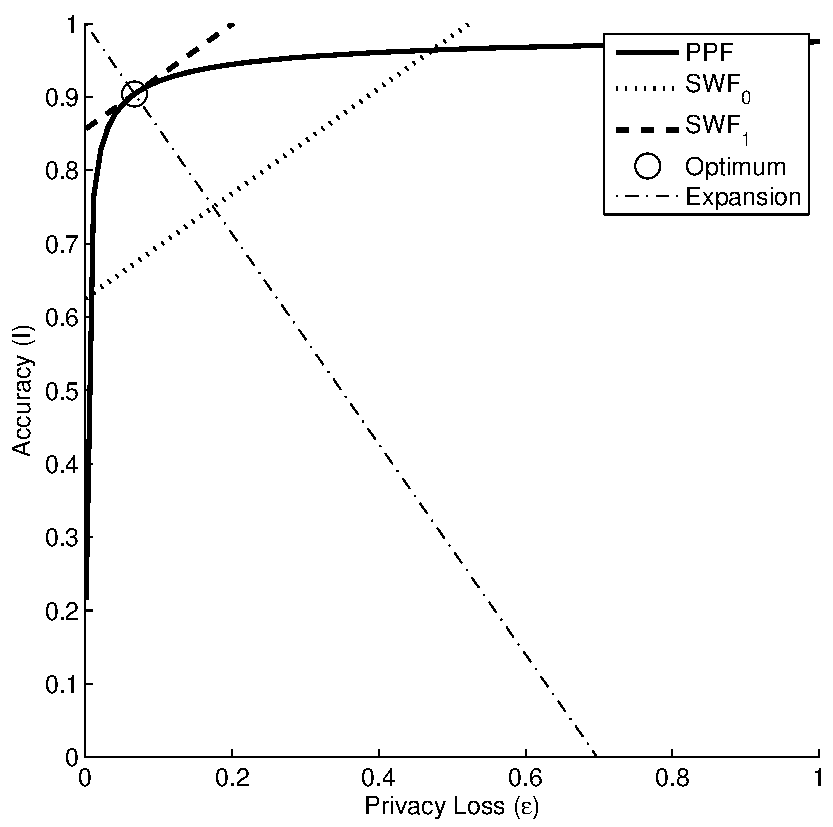
\includegraphics[scale=.5]{plannersprob_income}
\end{center}


%TCIMACRO{\TeXButton{EndFrame}{\end{frame}}}%
%BeginExpansion
\end{frame}%
%EndExpansion
%
%%%%%%%%%%%%%%%%%%%%%%%%%%%%%%%%%%%%%%%%%%%%%%%%%%%%%%%%%%%%%%%%%
%%%%%%%%%%%%%%%%%%%%%%%%%%%%%%%%%%%%%%%%%%%%%%%%%%%%%%%%%%%%%%%%%



%%%%%%%%%%%%%%%%%%%%%%%%%%%%%%%%%%%%%%%%%%%%%%%%%%%%%%%%%%%%%%%%%
%%%%%%%%%%%%%%%%%%%%%%%%%%%%%%%%%%%%%%%%%%%%%%%%%%%%%%%%%%%%%%%%%
%TCIMACRO{\TeXButton{BeginFrame}{\begin{frame}[allowframebreaks]}}%
%BeginExpansion
\begin{frame}[allowframebreaks]%
%EndExpansion
\frametitle{Application: Health Status}
\textbf{Preferences:}
\begin{equation}
\begin{array}{l}
v\left( y_{i},\varepsilon ,I,h_{i},p\right) = \\
-\sum_{\ell =1}^{L}\xi _{\ell }\ln p_{\ell }+\ln y_{i}-\func{E}\left[ \gamma
_{i}\right] \varepsilon -\left( \gamma _{i}-\func{E}\left[ \gamma _{i}\right]
\right) \left( 1-\ln h_{i}\right) \varepsilon  \\
+\func{E}\left[ \eta _{i}\right] I+\left( \eta _{i}-\func{E}\left[ \eta _{i}%
\right] \right) \ln y_{i}I%
\end{array}
%\label{eqn:linear_health}
\end{equation}%

%TCIMACRO{\TeXButton{EndFrame}{\end{frame}}}%
%BeginExpansion
\end{frame}%
%EndExpansion
%
%%%%%%%%%%%%%%%%%%%%%%%%%%%%%%%%%%%%%%%%%%%%%%%%%%%%%%%%%%%%%%%%%
%%%%%%%%%%%%%%%%%%%%%%%%%%%%%%%%%%%%%%%%%%%%%%%%%%%%%%%%%%%%%%%%%

%%%%%%%%%%%%%%%%%%%%%%%%%%%%%%%%%%%%%%%%%%%%%%%%%%%%%%%%%%%%%%%%%
%%%%%%%%%%%%%%%%%%%%%%%%%%%%%%%%%%%%%%%%%%%%%%%%%%%%%%%%%%%%%%%%%
%TCIMACRO{\TeXButton{BeginFrame}{\begin{frame}[allowframebreaks]}}%
%BeginExpansion
\begin{frame}[allowframebreaks]%
%EndExpansion
\frametitle{Data}
Cornell National Social Survey (CNSS) from 2011, 2012,
and 2013.
\begin{itemize}
\item Income, measured in nine bins;

\item \texttt{JAq6}, \textquotedblleft In general, how would you rate your
overall health?\textquotedblright\

\item \textquotedblleft If medical information could be shared
electronically between the places where a patient receives medical care, how
do you think that would:\textquotedblright\

\begin{enumerate}
\item \texttt{JAq4@b}, \textquotedblleft \ldots affect the privacy and
security of medical information?\textquotedblright\ measured as a Likert
scale with five categories (proxy for privacy preferences, $\gamma $).

\item \texttt{JAq4@a}, \textquotedblleft \ldots affect the quality of
medical care?\textquotedblright\ measured as a Likert scale with five
categories (proxy for accuracy preferences, $\eta $).
\end{enumerate}

\end{itemize}

%TCIMACRO{\TeXButton{EndFrame}{\end{frame}}}%
%BeginExpansion
\end{frame}%
%EndExpansion
%
%%%%%%%%%%%%%%%%%%%%%%%%%%%%%%%%%%%%%%%%%%%%%%%%%%%%%%%%%%%%%%%%%
%%%%%%%%%%%%%%%%%%%%%%%%%%%%%%%%%%%%%%%%%%%%%%%%%%%%%%%%%%%%%%%%%

%%%%%%%%%%%%%%%%%%%%%%%%%%%%%%%%%%%%%%%%%%%%%%%%%%%%%%%%%%%%%%%%%
%%%%%%%%%%%%%%%%%%%%%%%%%%%%%%%%%%%%%%%%%%%%%%%%%%%%%%%%%%%%%%%%%
%TCIMACRO{\TeXButton{BeginFrame}{\begin{frame}[allowframebreaks]}}%
%BeginExpansion
\begin{frame}[allowframebreaks]%
%EndExpansion
\frametitle{Measurement}
\begin{itemize}
\item $\limfunc{Corr}\left[ \gamma _{i},\ln h_{i}\right] =0.015\left( \pm
0.021\right) $

\item $\limfunc{Corr}\left[ \gamma _{i},\ln y_{i}\right] =0.009\left( \pm
0.020\right) $

\item $\limfunc{Corr}\left[ \eta _{i},\ln y_{i}\right] =0.176\left( \pm
0.020\right) $
\end{itemize}

%TCIMACRO{\TeXButton{EndFrame}{\end{frame}}}%
%BeginExpansion
\end{frame}%
%EndExpansion
%
%%%%%%%%%%%%%%%%%%%%%%%%%%%%%%%%%%%%%%%%%%%%%%%%%%%%%%%%%%%%%%%%%
%%%%%%%%%%%%%%%%%%%%%%%%%%%%%%%%%%%%%%%%%%%%%%%%%%%%%%%%%%%%%%%%%

%%%%%%%%%%%%%%%%%%%%%%%%%%%%%%%%%%%%%%%%%%%%%%%%%%%%%%%%%%%%%%%%%
%%%%%%%%%%%%%%%%%%%%%%%%%%%%%%%%%%%%%%%%%%%%%%%%%%%%%%%%%%%%%%%%%
%TCIMACRO{\TeXButton{BeginFrame}{\begin{frame}[allowframebreaks]}}%
%BeginExpansion
\begin{frame}[allowframebreaks]%
%EndExpansion
\frametitle{Implications}
\begin{equation*}
MRT\left( \varepsilon ^{0},I^{0}\right) =0.837
\end{equation*}%
\begin{itemize}
	\item Welfare loss: a 2 percent decrease in accuracy requires an 0.6 percent increase in income.
\end{itemize}
%TCIMACRO{\TeXButton{EndFrame}{\end{frame}}}%
%BeginExpansion
\end{frame}%
%EndExpansion
%
%%%%%%%%%%%%%%%%%%%%%%%%%%%%%%%%%%%%%%%%%%%%%%%%%%%%%%%%%%%%%%%%%
%%%%%%%%%%%%%%%%%%%%%%%%%%%%%%%%%%%%%%%%%%%%%%%%%%%%%%%%%%%%%%%%%




% %%%%%%%%%%%%%%%%%%%%%%%%%%%%%%%%%%%%%%%%%%%%%%%%%%%%%%%%%%%%%%%%%
% %%%%%%%%%%%%%%%%%%%%%%%%%%%%%%%%%%%%%%%%%%%%%%%%%%%%%%%%%%%%%%%%%
% %TCIMACRO{\TeXButton{BeginFrame}{\begin{frame}[allowframebreaks]}}%
% %BeginExpansion
% \begin{frame}[allowframebreaks]%
% %EndExpansion
% \frametitle{}

% %TCIMACRO{\TeXButton{EndFrame}{\end{frame}}}%
% %BeginExpansion
% \end{frame}%
% %EndExpansion
% %
% %%%%%%%%%%%%%%%%%%%%%%%%%%%%%%%%%%%%%%%%%%%%%%%%%%%%%%%%%%%%%%%%%
% %%%%%%%%%%%%%%%%%%%%%%%%%%%%%%%%%%%%%%%%%%%%%%%%%%%%%%%%%%%%%%%%% 